\chapter{Threat Model} \label{ch:threat-model}
This chapter contains the threat model established for the system under scrutiny, which was used to identify and document all threats to the system. The methodology and threat model technique is described in section \ref{ch:method:threat-modeling}.

\section{Assets}
As part of the first phase of our threat modeling technique, assets of the system were identified. These can be found in table \ref{tb:assets}.
\begin{table}[!ht]
    \centering
    \begin{tabular}{r l}
        \hline
        \textbf{ID} & \textbf{Description} \\
        \hline
        1  & Physical access to the house \\
        2  & Personal four digit pin \\
        3  & Arm/disarm state of the system \\
        4  & Door contact sensor state \\
        5  & Authentication to the admin web application \\
        6  & Triggered alarm state \\
        7  & [TODO...] \\
        \hline
    \end{tabular}
    \caption{The identified assets of the system}
    \label{tb:assets}
\end{table}

\section{Use cases}
\begin{table}[!ht]
    \centering
    \begin{tabularx}{\textwidth}{r X}
        \textbf{ID} & \textbf{Description}  \\
        \hline
        1  & The user arms/disarms the system via the remote keypad panel \\
        2  & The user arms/disarms the system via the web portal \\
        3  & The user arms/disarms the system via the mobile app \\
        4  & The user receives a notification about a state change in the system \\
        5  & [TODO...] \\
        \hline
    \end{tabularx}
    \caption{Use cases of the system}
    \label{tb:use-cases}
\end{table}

\section{System Architecture}

\subsection{System Technologies}
\begin{table}[!ht]
    \centering
    \begin{tabularx}{\textwidth}{l X}
        \textbf{Technology}  & \textbf{Description} \\
        \hline
        Main Panel & Linux 2.6-2.30. Hosts a web server over HTTP, using Mongoose (an embedded web server), version unknown. Unknown application listening on TCP port 58098. Hosts DNS on TCP/UDP port 53. Has a USB and ethernet port. \\
        \hline
        HTTP  & Protocol used by the admin web application. A clear text protocol, used to communicate with the web admin panel. \\
        \hline
        F1 RF protocol  & A proprietary \gls{RF} protocol from the hardware manufacturer, Climax Technology. Uses 868 MHz frequency. Completely undocumented. \\
        \hline
        Mongoose web server  & An open source web server, in C. Used by the main panel to host the local admin web page, version unknown. \\
        \hline
    \end{tabularx}
    \caption{Technologies used in the system}
    \label{tb:system-technologies}
\end{table}

\subsection{Overview of The System Architecture}
\begin{figure}[!ht]
    \centering
    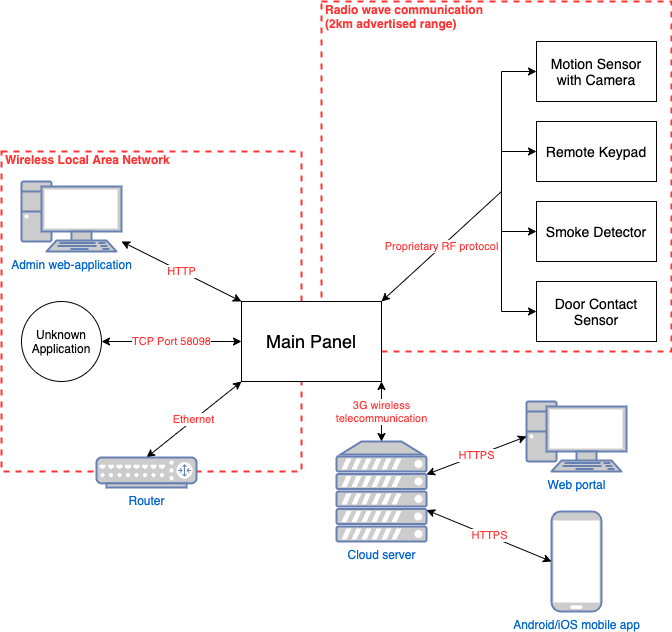
\includegraphics[width=\textwidth]{images/system-overview.png}
    \caption{Overview of the System Architecture}
    \label{fig:system-overview}
\end{figure}
